 \documentclass[journal]{IEEEtran}   

\usepackage[utf8]{inputenc}
\usepackage[T1]{fontenc}
\usepackage{cite}
\usepackage{hyperref} 
\usepackage{amsmath}
\usepackage{tikz}
\usepackage{listings}
\lstset{language=Python, basicstyle=\ttfamily\scriptsize, breaklines=true, frame=single, columns=fullflexible, keepspaces=true, showstringspaces=false}
\usetikzlibrary{arrows.meta, positioning, calc, shapes.multipart}
\usetikzlibrary{backgrounds}

\title{\LARGE \bf
Modelo de IA para evaluar el riesgo en sitios web y detección de posibles sitios web de Phishing
}

\author{
Juan David Orduz Sastoque - 20221020096\par
Universidad Distrital Francisco José de Caldas\par
Facultad de Ingeniería}


\begin{document}

\maketitle
\thispagestyle{empty}
\pagestyle{empty}

\section{RESUMEN}
El phishing sigue creciendo porque se centra en atacar a la persona, no al sistema, y las listas negras siempre llegan tarde, ya que cuando un sitio nuevo aparece reportado, ya cumplió su objetivo. Frente a esto, el proyecto propone un agente de IA que reciba una URL y estime su riesgo de phishing sin depender de esas listas, analizando en su lugar rasgos de la URL y el dominio (longitud, caracteres raros, IP en vez de dominio, edad de registro) y, cuando el sitio sea accesible, elementos del contenido como formularios de login o similitud con marcas conocidas. Para el modelo se utilizará XGBoost, Random Forest y LightGBM con el fin de promediar la importancia que cada uno asigna a las variables y quedarse con las más relevantes, pues sobre ese conjunto reducido se construirá un stacking de dos niveles, donde XGBoost y Random Forest generan cada uno una probabilidad de phishing que alimenta a un segundo XGBoost más simple encargado de la predicción final. Todo se entrenará con URLs reales de sitios de phishing y de sitios legítimos recolectadas de fuentes públicas, de modo que el agente reciba una URL cruda y no características ya calculadas. La meta es entregar un agente que funcione y claridad sobre los límites referente a qué tanto generaliza a sitios nuevos y qué tan fácil es engañarlo con URLs hechas para evadirlo.
\newline \par
\textbf{Palabras Clave:} Phishing, Ciberseguridad, Inteligencia Artificial, Aprendizaje Automático, Detección de URL, Análisis de Riesgo, Ensambles, Explicabilidad.
    

\section{abstract}
    Phishing continues to grow because it targets the individual rather than the system. Furthermore, blacklists are inherently reactive—by the time a new site is reported, it has already achieved its objective. To address this, the project proposes an AI agent that evaluates the phishing risk of a given URL without relying on such lists. Instead, it analyzes characteristics of the URL and its domain—such as length, the presence of unusual characters, the use of an IP address rather than a domain name, and the domain's registration age. When a site is accessible, the agent also examines content elements, including login forms or visual similarities to well-known brands. The model employs XGBoost, Random Forest, and LightGBM to assess the relative importance of various features, retaining only the most significant ones. This refined subset of features serves as the foundation for a two-level stacking architecture: XGBoost and Random Forest each generate a phishing probability, which then feeds into a simpler, second-level XGBoost model responsible for the final prediction. The system is trained on a dataset of real phishing and legitimate URLs gathered from public sources, allowing the agent to process raw URLs directly rather than relying on pre-calculated features. The goal is to provide a functional agent, while also offering clarity regarding its limitations specifically, how well it generalizes to new, previously unseen sites and how susceptible it might be to evasion tactics using specially crafted URLs.
\newline \par

\textbf{Keywords:} Phishing, Cybersecurity, Artificial Intelligence, Machine Learning, URL Analysis, Risk Assessment, Ensemble Learning, Explainability.


\section{INTRODUCCIÓN}

 Detectar phishing con reglas fijas tiene un problema de fondo y es que las reglas se pueden aprender y evadir. Por eso gran parte de la investigación de la última década se centró en el aprendizaje automático, que en lugar de comparar contra una lista aprende patrones a partir de miles de ejemplos etiquetados. Los primeros enfoques de este tipo se apoyaron casi por completo en características léxicas extraídas directamente de la URL como la longitud, número de puntosy presencia de palabras sospechosas, combinadas con clasificadores clásicos como Random Forest o SVM, y llegaron a superar el 97\% de exactitud usando conjuntos de datos de más de 70.000 URLs \cite{sahingoz2019machine}. Otros trabajos sumaron a esas características léxicas información obtenida del código fuente y de servicios de terceros como la edad del dominio, certificados o reputación, lo que llevó la exactitud hasta 99,31\% con Random Forest \cite{rao2019detection}. El problema de tener demasiadas variables, muchas de ellas redundantes, motivó el desarrollo de esquemas de selección de características por ensamble, donde uno de ellos logró distinguir el 94,6\% de los sitios usando solo el 20,8\% de las características originales \cite{chiew2019hybrid}, mientras que otro combinó esa selección con una red neuronal para obtener un modelo más compacto sin perder desempeño \cite{zhu2019ofsnn}. En paralelo surgieron modelos que evitan por completo la ingeniería manual de características, procesando la URL carácter por carácter mediante redes convolucionales \cite{aljofey2020effective}. \newline

Sobre esa base, la investigación más reciente se movió hacia arquitecturas de apilamiento con modelos de apilamiento en múltiples capas, que combinan clasificadores como MLP, KNN, Random Forest, Regresión Logística y XGBoost organizados en capas donde la salida de una alimenta a la siguiente, estas arquitecturas alcanzaron entre 96,79\% y 98,90\% de exactitud sobre distintos datasets de phishing \cite{kalabarige2022multilayer}, y una versión posterior de ese mismo enfoque, pero reemplazando los clasificadores base por algoritmos de boosting y sumando una etapa de selección de características por importancia promedio, mostró que reducir las variables a un 66-86\% del total no perjudica el desempeño, e incluso lo mejora en algunos casos \cite{kalabarige2023boosting}. Así mismo se ha explorado mantener fijo un solo algoritmo base y variar la estrategia de meta aprendizaje (AdaBoost, Bagging, Rotation Forest, LogitBoost), lo que también supera el 97\% de exactitud con tasas de falsos positivos por debajo de 0,03 y deja claro que tanto el clasificador base como la técnica de ensamble influyen en el resultado final \cite{alsariera2020ai}. Sin embargo, la exactitud reportada en estos trabajos no cuenta toda la historia, pues se ha demostrado que modelos como SVM caen a una tasa de detección de apenas 10\% frente a URLs generadas deliberadamente para evadirlos, mientras que los enfoques multimodales, que combinan dominio, HTML y contenido visual, resisten mucho mejor, con detección cercana al 99\% \cite{duy2024study}, y una revisión reciente de más de 130 artículos publicados entre 2020 y 2024 señala que buena parte de los modelos actuales siguen entrenados sobre datasets fijos y con extracción de características poco dinámica, lo que limita su capacidad de adaptarse a técnicas de phishing nuevas \cite{ahmad2025across}. En conjunto, estos trabajos confirman que los ensambles y el stacking superan a los clasificadores individuales, que la selección de características puede reducir el costo computacional sin sacrificar exactitud, y que ningún modelo está exento de ser evadido si no se piensa también en su robustez frente a ataques adversarios.

\section{TRABAJOS RELACIONADOS}

En el primer trabajo de Kalabarige, la metodología parte de una selección híbrida de características, pues se entrenan tres algoritmos de boosting (XGBoost, CatBoost y LightGBM), se extrae la importancia que cada uno le asigna a las variables, se promedia esa importancia entre los tres modelos y se conservan las K variables mejor puntuadas, con K variando entre el 66\% y el 86\% del total según el dataset. Sobre ese subconjunto de características se entrena un modelo de apilamiento de tres capas construido con algoritmos de boosting, donde la primera capa usa XGBoost, LightGBM, CatBoost y AdaBoost, la segunda descarta AdaBoost y conserva los tres restantes, y la tercera usa XGBoost como meta aprendiz final. El proceso se repite en cuatro fases, con todas las características sin balanceo, con las K seleccionadas, sin balanceo y ambas variantes con balanceo mediante sobremuestreo aleatorio para medir el efecto de cada decisión por separado \cite{kalabarige2023boosting}. \newline

En el trabajo previo de los mismos autores, la metodología es más sencilla en cuanto a la etapa de features, ya que no hay selección, sino que se usan todas las variables del dataset. El aporte metodológico está en la arquitectura de apilamiento, pues la primera capa combina cinco clasificadores heterogéneos (MLP, KNN, Random Forest, Regresión Logística y XGBoost), de esos cinco se seleccionan los tres de mejor desempeño para conformar la segunda capa, y la tercera usa nuevamente XGBoost como meta aprendiz. Antes de entrenar, los datasets con clases desbalanceadas se balancean mediante sobremuestreo aleatorio (ROS), duplicando instancias de la clase minoritaria hasta igualarla con la mayoritaria, y el modelo se evalúa comparando su desempeño con y sin ese balanceo \cite{kalabarige2022multilayer}. \newline

Duy aborda la metodología desde un ángulo distinto, centrado en poner a prueba la robustez de los modelos más que en optimizar su exactitud. Por lo que construyen un framework llamado AWG que combina una red generativa adversaria tipo Wasserstein con un algoritmo de generación de dominios maliciosos (Charbot), de forma que un generador aprende a producir URLs adversarias que engañan a un discriminador entrenado para imitar el comportamiento de un detector de caja negra. Con las muestras generadas atacan quince modelos distintos, de tipo ML, ensamble, aprendizaje profundo y multimodal, bajo un escenario de ataque de transferencia, donde el atacante no conoce la arquitectura interna del modelo víctima. Como segunda etapa metodológica, proponen una estrategia de defensa por reentrenamiento, donde seleccionan las muestras adversarias de mayor calidad (las que lograron evadir un clasificador de dominios) y las mezclan con el dataset original para reentrenar los modelos víctima, midiendo la mejora en su tasa de detección \cite{duy2024study}. \newline

Ahmad no propone un modelo propio, sino que su metodología es la de una revisión sistemática de literatura. Parten de una búsqueda con la palabra clave "Web Phishing Detection", que arrojó cerca de 3,500 artículos, de esos artículos van filtrando por especificidad y por año de publicación (2020-2024) hasta quedarse con 150 artículos, divididos en 100 de investigación original, 30 encuestas y 20 revisiones. Sobre ese conjunto organizan la información en categorías, modos de ataque, técnicas de detección basadas en listas, en heurísticas, en el lado del cliente y en modelos de IA, y comparan el desempeño reportado por cada estudio usando la exactitud como métrica común, lo que les permite construir un mapa comparativo de qué modelos y qué técnicas de extracción de características han dado mejores resultados en la literatura reciente \cite{ahmad2025across}. \newline

Por último, Alsariera fija un único algoritmo base (Extra-Trees) y varían la estrategia de meta aprendizaje sobre él, dando lugar a cuatro modelos, AdaBoost-Extra Tree, Bagging-Extra Tree, Rotation Forest-Extra Tree y LogitBoost-Extra Tree. Los cuatro se entrenan y validan mediante validación cruzada de 10 particiones sobre el dataset de phishing de UCI, particionando los datos en diez grupos, entrenando sobre nueve y probando sobre el restante en cada iteración. El desempeño de cada modelo se mide con exactitud, tasa de falsos positivos, tasa de falsos negativos y F-measure, y luego se compara contra quince métodos previos publicados entre 2014 y 2020 para ubicar los resultados dentro del estado del arte \cite{alsariera2020ai}. \newline

La metodología de este proyecto se apoya en el enfoque de Kalabarige \cite{kalabarige2023boosting} de usar varios modelos de boosting para promediar la importancia de las variables antes de entrenar el modelo final, pero la simplifica a una sola capa de apilamiento, con XGBoost y Random Forest como clasificadores base y un segundo XGBoost como meta clasificador. El detalle completo del pipeline, del proceso de entrenamiento y de la estrategia de evaluación se desarrolla en la siguiente sección.

\section{METODOLOGÍA}

El pipeline propuesto se muestra en la Figura~\ref{fig:arquitectura}. Recibe como entrada una URL y, cuando el sitio está accesible, extrae características, calcula la importancia promedio de esas características con tres modelos de boosting, conserva solo las más relevantes, y las pasa a un stacking de dos niveles cuya salida final viene acompañada de una explicación generada con SHAP.

\begin{figure}[t]
\centering
\resizebox{\linewidth}{!}{%
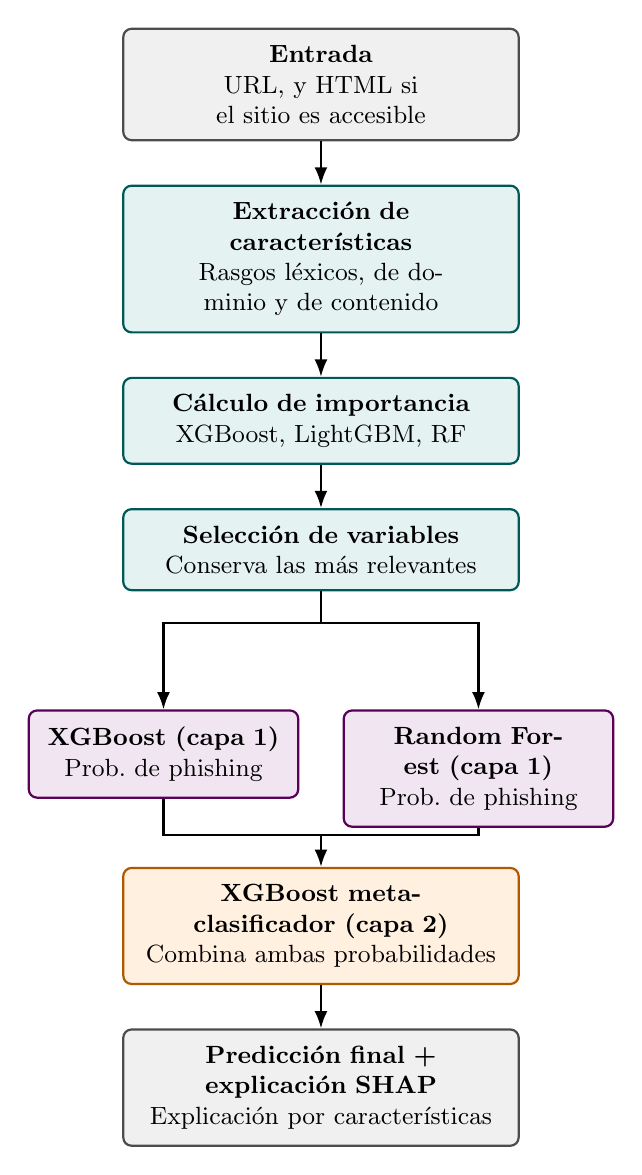
\begin{tikzpicture}[
    node distance=0.55cm,
    every node/.style={font=\small},
    box/.style={
        rectangle, rounded corners=3pt, draw, thick,
        text width=4.6cm, align=center, minimum height=1cm,
        inner sep=6pt
    },
    boxsmall/.style={
        rectangle, rounded corners=3pt, draw, thick,
        text width=3.0cm, align=center, minimum height=1cm,
        inner sep=6pt
    },
    gray/.style={box, fill=gray!12, draw=gray!60!black},
    teal/.style={box, fill=teal!10, draw=teal!70!black},
    purple/.style={boxsmall, fill=violet!10, draw=violet!70!black},
    coral/.style={box, fill=orange!12, draw=orange!70!black},
    arrow/.style={-{Latex[length=2.2mm]}, thick}
]

% --- Nodos ---
\node[gray] (input) {\textbf{Entrada}\\ URL, y HTML si el sitio es accesible};

\node[teal, below=of input] (features)
    {\textbf{Extracción de características}\\ Rasgos léxicos, de dominio y de contenido};

\node[teal, below=of features] (importance)
    {\textbf{Cálculo de importancia}\\ XGBoost, LightGBM, RF};

\node[teal, below=of importance] (selection)
    {\textbf{Selección de variables}\\ Conserva las más relevantes};

\node[purple, below=1.5cm of selection, xshift=-2.0cm] (xgb1)
    {\textbf{XGBoost (capa 1)}\\ Prob.\ de phishing};

\node[purple, below=1.5cm of selection, xshift=2.0cm] (rf1)
    {\textbf{Random Forest (capa 1)}\\ Prob.\ de phishing};

\node[coral, below=3.5cm of selection] (meta)
    {\textbf{XGBoost meta-clasificador (capa 2)}\\ Combina ambas probabilidades};

\node[gray, below=of meta] (output)
    {\textbf{Predicción final + explicación SHAP}\\ Explicación por características};

% --- Flechas ---
\draw[arrow] (input) -- (features);
\draw[arrow] (features) -- (importance);
\draw[arrow] (importance) -- (selection);

\draw[arrow] (selection.south) -- ++(0,-0.4) -| (xgb1.north);
\draw[arrow] (selection.south) -- ++(0,-0.4) -| (rf1.north);

\coordinate (merge) at ($(meta.north)+(0,0.4)$);
\draw[thick] (xgb1.south) -- (xgb1.south |- merge) -- (merge);
\draw[thick] (rf1.south) -- (rf1.south |- merge) -- (merge);
\draw[arrow] (merge) -- (meta.north);

\draw[arrow] (meta) -- (output);

\end{tikzpicture}}
\caption{Arquitectura del modelo de stacking de dos niveles propuesto para la detección de phishing.}
\label{fig:arquitectura}
\end{figure}

\subsection{Datos}

Para entrenar el modelo se construirá un dataset a partir de URLs crudas, de modo que el agente reciba una dirección y no un vector de características ya calculado, como ocurre con el dataset de UCI \cite{alsariera2020ai}, que distribuye únicamente las variables. Las URLs de phishing se tomarán de feeds públicos como PhishTank y OpenPhish, y las legítimas de la lista Tranco \cite{lepochat2019tranco}, un ranking de sitios populares pensado para investigación y más difícil de manipular que el de Alexa, que dejó de existir en 2022. Estas fuentes de phishing, junto con un ranking de sitios populares para los legítimos, ya fueron usadas en \cite{duy2024study}. Se recolectará un número similar de URLs por clase, se eliminarán los duplicados y se registrará la fecha de captura de cada URL, porque los sitios de phishing tienen una vida corta y muchos dejan de estar disponibles pocas horas después de reportarse.

Como Tranco solo lista dominios, las URLs legítimas se completarán con rutas internas tomadas de la página principal de cada sitio, para que el modelo no aprenda a asociar la presencia de una ruta con phishing. Al muestrear las clases en igual proporción no se espera necesitar balanceo, si aun así quedara desbalance, se aplicará sobremuestreo aleatorio (ROS) solo sobre las particiones de entrenamiento, siguiendo el procedimiento de \cite{kalabarige2022multilayer}. Como los trabajos \cite{kalabarige2022multilayer}, \cite{kalabarige2023boosting} y \cite{alsariera2020ai} usan otros conjuntos de datos, sus exactitudes no son directamente comparables con las de este proyecto. Por eso la comparación con ellos será cualitativa, y la cuantitativa se hará contra los clasificadores base entrenados sobre este mismo dataset.

\subsection{Extracción de características}

De la URL se extraen rasgos léxicos y de dominio como la longitud total, número de puntos, presencia de una dirección IP en lugar de un nombre de dominio, uso del carácter ```@' o de guiones, uso de HTTPS y edad de registro del dominio cuando esté disponible. Cuando el sitio sea accesible, se suman elementos del HTML como la presencia de formularios de inicio de sesión, número y origen de scripts embebidos, y enlaces externos. Como las características se calculan directamente desde las URLs del dataset, el mismo código de extracción sirve en el entrenamiento y en la predicción sobre una URL nueva, lo que evita el desajuste entre ambos. Dado que muchos sitios de phishing ya no están en línea cuando se intenta descargarlos, el HTML se descargará en el momento de recolectar cada URL, y las características que no puedan calcularse (HTML o WHOIS no disponibles) se codificarán con un valor centinela, para que el modelo aprenda a trabajar también con URLs de las que solo se conoce la dirección. Este conjunto de características es deliberadamente más reducido que el de trabajos como \cite{kalabarige2023boosting}, que llega a manejar 111 variables; la apuesta aquí es que un conjunto más chico, bien seleccionado, sea suficiente para un agente que necesita responder rápido sobre una URL nueva.

\subsection{Selección de características por importancia promedio}

Sobre el conjunto de características extraídas se entrenan tres modelos XGBoost, LightGBM y Random Forest, con el único propósito de obtener la importancia que cada uno asigna a cada variable. Siguiendo el esquema de \cite{kalabarige2023boosting}, esa importancia se promedia entre los tres modelos:

\begin{equation*}
AVG_{F_i} = \frac{1}{3} \sum_{j=1}^{3} RF_{i}^{j}
\end{equation*}

Donde $RF_{i}^{j}$ es la importancia de la característica $i$ según el modelo $j$. Las características se ordenan por ese promedio y se conservan las $K$ de mayor puntaje; el valor de $K$ se determinará experimentalmente, evaluando la exactitud del modelo final en un rango de valores (por ejemplo, reteniendo entre el 60\% y el 90\% del total de variables) y quedándose con el punto donde la exactitud deja de mejorar de forma apreciable.

\subsection{Arquitectura del modelo}

El modelo final es un stacking de dos niveles, como se ve en la Figura~\ref{fig:arquitectura}. En la primera capa, XGBoost y Random Forest se entrenan en paralelo sobre las características seleccionadas, cada uno entrega, para una URL dada, la probabilidad de que sea phishing. Esas dos probabilidades, no las etiquetas finales, se concatenan y se usan como entrada de un segundo XGBoost, más simple, que actúa como meta clasificador y entrega la predicción final. Esta arquitectura usa una capa menos que las tres de BMLSELM \cite{kalabarige2023boosting}, apostando a que dos modelos bien diferenciados en cómo cometen errores, uno basado en boosting secuencial, otro en promediado de árboles independientes, aportan suficiente diversidad sin necesitar una tercera capa intermedia.

\subsection{Entrenamiento y validación}

El entrenamiento se hará con validación cruzada de 10 particiones, siguiendo el esquema usado en \cite{alsariera2020ai}, donde los datos se dividen en diez grupos, se entrena sobre nueve y se prueba sobre el restante, repitiendo el proceso diez veces para que cada partición sirva de test exactamente una vez. A diferencia de \cite{alsariera2020ai}, las particiones se construirán agrupando las URLs por dominio, de modo que URLs de un mismo dominio no queden a la vez en entrenamiento y en prueba, pues de lo contrario el modelo podría memorizar dominios y sobrestimar su capacidad de generalizar a sitios nuevos. Por la misma razón, la selección de características y el balanceo se calcularán únicamente con la partición de entrenamiento de cada iteración. Los hiperparámetros de cada modelo (profundidad máxima de los árboles, tasa de aprendizaje, número de estimadores) se ajustarán mediante búsqueda en grilla sobre el conjunto de entrenamiento, evitando así que la selección de hiperparámetros contamine la evaluación final.

\subsection{Explicabilidad}

Sobre el meta clasificador final se aplicará SHAP para generar dos tipos de explicación, una explicación global, que muestra qué características pesan más en promedio sobre todo el dataset, y una explicación local, que para una URL puntual muestra qué características empujaron la decisión hacia ``phishing'' o ``legítimo'' y en qué magnitud. Esta segunda es la que responde directamente al objetivo de que la evaluación de riesgo venga acompañada de una justificación.

\subsection{Evaluación}

El desempeño del modelo se medirá con las métricas estándar de la literatura revisada correspondientes a exactitud, precisión, recall, F1-score y tasa de falsos positivos, siguiendo las definiciones usadas en \cite{kalabarige2023boosting} y \cite{alsariera2020ai}. Además de reportar estas métricas para el stacking completo, se entrenará cada clasificador base (XGBoost solo, Random Forest solo) de forma aislada sobre el mismo conjunto de datos, para poder mostrar cuánto aporta realmente la arquitectura de dos capas frente a usar un solo modelo. Finalmente, como una primera aproximación a la robustez del agente, inspirada en el trabajo de Duy \cite{duy2024study}, se probará el modelo contra un pequeño conjunto de URLs modificadas manualmente para imitar técnicas de evasión simples (cambios menores en el dominio, uso de acortadores de URL, subdominios adicionales), con el fin de reportar de forma honesta qué tan fácil es engañar al agente, sin llegar a implementar un framework de generación adversaria completo como el de ese trabajo.


\section{DISEÑO E IMPLEMENTACIÓN}

La Metodología describe qué modelo se entrena y con qué datos. Esta sección describe cómo se construye, alrededor de ese modelo, un sistema que alguien pueda usar, algo que reciba una URL cualquiera y devuelva un veredicto con su justificación. Un clasificador con buena exactitud sobre un archivo de datos todavía no es un agente, ya que aún falta la parte que descarga la página sin ponerse en riesgo, calcula las mismas características que se usaron al entrenar, aplica el modelo y presenta el resultado de forma legible. \newline

Esta sección tiene dos partes, en el Diseño se define el sistema de manera casi independiente de la herramienta, con sus componentes, clases, el recorrido de una URL, el formato de la respuesta y las medidas de seguridad. En este apartado se usan tres diagramas UML (componentes, clases y secuencia) porque cada uno responde una pregunta distinta, que ayuda a comprender mejor el modelo, qué piezas hay y dónde corren, cómo se reparten las responsabilidades y en qué orden se comunican. En Implementación se describe cómo se materializa ese diseño en Google Colab, Colab condiciona el diseño en un punto, pues no ofrece un servicio permanente, y cada sesión es una máquina virtual efímera. Por eso el agente se plantea como una función que se invoca desde el notebook, y todo lo que debe sobrevivir entre sesiones (dataset, modelo entrenado, lista de variables seleccionadas) se guarda en Google Drive y se carga al iniciar.

\subsection{Diseño}

\subsubsection{Arquitectura General} 

La FiguraFigura~\ref{fig:componentes} muestra el sistema como un conjunto de componentes que corren dentro de un único entorno, el runtime de Google Colab. El camino principal tiene cinco componentes, la interfaz del agente recibe la URL del usuario, la adquisición descarga el HTML y consulta WHOIS, la extracción convierte lo descargado en un vector de características, la predicción selecciona las variables relevantes y calcula la probabilidad de phishing, y la explicación e informe genera las contribuciones SHAP y arma la respuesta. Las flechas continuas son el flujo de datos de ese camino, y las discontinuas indican que un componente usa un recurso externo. \newline

El diseño separa a propósito la adquisición de la extracción. Solo el componente de adquisición toca la red y el contenido no confiable del sitio. Todo lo demás trabaja con datos ya descargados, lo que concentra en un solo lugar el riesgo de analizar páginas sospechosas. \newline

Hay también un componente de entrenamiento que corre fuera de línea. Reutiliza el mismo componente de extracción que el camino principal, de modo que las características calculadas al entrenar y al predecir salen del mismo código, y evita el desajuste entre ambos. Lee el dataset desde Google Drive y escribe allí los artefactos del modelo, que el componente de predicción carga al iniciar. Drive se dibuja fuera de la frontera de Colab porque es almacenamiento persistente, independiente de la máquina virtual efímera.
\newline


\begin{figure*}[ht]
\centering
\resizebox{\textwidth}{!}{%
\begin{tikzpicture}[
    font=\footnotesize,
    comp/.style={rectangle, rounded corners=3pt, draw, thick, text width=2.4cm, align=center, minimum height=1.5cm, inner sep=4pt},
    ext/.style={rectangle, rounded corners=3pt, draw, thick, text width=2.2cm, align=center, minimum height=1.0cm, inner sep=4pt, fill=gray!12, draw=gray!60!black},
    verde/.style={comp, fill=teal!10, draw=teal!70!black},
    lila/.style={comp, fill=violet!10, draw=violet!70!black},
    naranja/.style={comp, fill=orange!12, draw=orange!70!black},
    gris/.style={comp, fill=gray!12, draw=gray!60!black},
    flecha/.style={-{Latex[length=2mm]}, thick},
    dep/.style={-{Latex[length=2mm]}, thick, dashed},
    et/.style={font=\scriptsize\itshape, inner sep=1.5pt}
]

    % Nodos Principales
    \node[ext] (user) at (-0.6,0) {\textbf{Usuario}\\ analista};
    \node[gris] (c1) at (3.6,0) {\textbf{Interfaz del agente}\\ {\scriptsize PhishingAgent}};
    \node[verde] (c2) at (7.2,0) {\textbf{Adquisición}\\ {\scriptsize URLFetcher}};
    \node[verde] (c3) at (10.8,0) {\textbf{Extracción}\\ {\scriptsize FeatureExtractor}};
    \node[lila] (c4) at (14.4,0) {\textbf{Predicción}\\ {\scriptsize FeatureSelector + StackingModel}};
    \node[lila] (c5) at (18.0,0) {\textbf{Explicación e informe}\\ {\scriptsize Explainer + RiskReport}};
    \node[naranja] (tr) at (10.8,-3.0) {\textbf{Entrenamiento}\\ {\scriptsize fit() fuera de línea}};
    \node (topspace) at (10.8,1.5) {};

    % Caja del Entorno Google Colab
    \begin{scope}[on background layer]
        \node[draw, dashed, thick, rounded corners=6pt, fill=gray!4, inner sep=10pt, fit=(c1)(c2)(c3)(c4)(c5)(tr)(topspace)] (colab) {};
    \end{scope}
    \node[font=\small\bfseries, anchor=north west] at ([xshift=10pt,yshift=-4pt]colab.north west) {Google Colab};

    % Recursos Externos
    \node[ext] (sitio) at (5.9,-5.4) {\textbf{Sitio objetivo}\\ HTTP(S)};
    \node[ext] (whois) at (8.6,-5.4) {\textbf{WHOIS / DNS}\\ servicio externo};
    \node[ext] (drive) at (14.4,-5.4) {\textbf{Google Drive}\\ dataset y artefactos};

    % Conexiones y Flujos de Datos
    \draw[flecha] (user) -- node[above, et]{URL} (c1);
    \draw[flecha] (c1) -- node[above, et]{URL} (c2);
    \draw[flecha] (c2) -- node[above, et]{página} (c3);
    \draw[flecha] (c3) -- node[above, et]{vector} (c4);
    \draw[flecha] (c4) -- node[above, et]{prob.} (c5);

    % Dependencias e Interacciones
    \coordinate (a1) at ($(c2.south)+(-0.5,0)$);
    \coordinate (a2) at ($(c2.south)+(0.5,0)$);
    \draw[dep] (a1) -- node[left, et]{GET} (a1 |- sitio.north);
    \draw[dep] (a2) -- node[right, et]{consulta} (a2 |- whois.north);
    \draw[dep] (tr.north) -- node[right, et]{reutiliza} (c3.south);
    \draw[flecha, <->] (tr.south) |- node[pos=0.25, left, et, align=right]{dataset /\\ artefactos} (drive.west);
    \draw[dep] (drive.north) -- node[right, et]{carga modelo} (c4.south);
    \draw[flecha] (c5.north) -- ++(0,1.9) -| node[pos=0.25, above, et]{RiskReport} (user.north);

\end{tikzpicture}}
\caption{Diagrama de componentes del agente. Las flechas continuas indican flujo de datos y las discontinuas, uso de un recurso externo o reutilización.}
\label{fig:componentes}
\end{figure*}

\subsubsection{Diseño de módulos}

La Figura~\ref{fig:clases} baja cada componente a clases concretas. PhishingAgent es el orquestador que posee una instancia de cada una de las otras cinco clases y expone un único método público, analyze(url), que devuelve un RiskReport. Su método privado validate\_url rechaza entradas inválidas antes de tocar la red, y el atributo risk\_thresholds guarda los umbrales que convierten la probabilidad en un nivel de riesgo. \newline

Cada una de las otras clases tiene una sola responsabilidad, URLFetcher descarga la página con límites de tiempo, tamaño y redirecciones, y verifica con is\_safe\_target que el destino sea aceptable. FeatureExtractor calcula las variables léxicas, de dominio y de HTML, y codifica con un valor centinela las que no pueden calcularse. FeatureSelector conserva las K variables de mayor importancia promedio. StackingModel encapsula las dos capas de XGBoost y Random Forest como base y un segundo XGBoost como meta-clasificador. Explainer calcula las contribuciones SHAP, y por eso depende de StackingModel. FeatureSelector y StackingModel tienen tanto fit como transform o predict\_proba, así que las mismas clases sirven para entrenar y para predecir. La página descargada y el vector de características se manejan como diccionarios simples y no como clases propias, para no inflar el diseño.
\newline


\begin{figure*}[ht]
\centering
\resizebox{\textwidth}{!}{%
\begin{tikzpicture}[
    font=\scriptsize,
    clase/.style={rectangle split, rectangle split parts=3, draw, thick,
                  text width=3.2cm, align=left, inner xsep=4pt, inner ysep=4pt,
                  rectangle split part fill={gray!18, white, white}},
    comp/.style={-{diamond[length=3.5mm, width=2.5mm]}, thick},
    uso/.style={-{Latex[length=2mm]}, thick, dashed},
    et/.style={font=\scriptsize\itshape, inner sep=2pt}
]

\node[clase] (agent) at (6.8,0)
  {\nodepart{one}\centering\textbf{PhishingAgent}
   \nodepart{two}- risk\_thresholds: dict
   \nodepart{three}+ analyze(url)\\- validate\_url(url)};

\node[clase] (report) at (13.6,0)
  {\nodepart{one}\centering\textbf{RiskReport}
   \nodepart{two}+ url, final\_url: str\\+ label: str\\+ probability: float\\+ risk\_level: str\\+ recommendation: str\\+ factors: list\\+ missing\_features: list\\+ model\_version: str
   \nodepart{three}+ to\_dict(): dict};

\node[clase] (fetch) at (0,-4.5)
  {\nodepart{one}\centering\textbf{URLFetcher}
   \nodepart{two}- timeout: float\\- max\_bytes: int\\- max\_redirects: int
   \nodepart{three}+ fetch(url): dict\\- is\_safe\_target(url)};

\node[clase] (extr) at (3.4,-4.5)
  {\nodepart{one}\centering\textbf{FeatureExtractor}
   \nodepart{two}- lexical\_features: list\\- html\_features: list\\- sentinel: int
   \nodepart{three}+ extract(url, page)};

\node[clase] (sel) at (6.8,-4.5)
  {\nodepart{one}\centering\textbf{FeatureSelector}
   \nodepart{two}- importances: dict\\- selected: list
   \nodepart{three}+ fit(X, y)\\+ transform(x)};

\node[clase] (model) at (10.2,-4.5)
  {\nodepart{one}\centering\textbf{StackingModel}
   \nodepart{two}- base\_xgb: XGB\\- base\_rf: RF\\- meta: XGB
   \nodepart{three}+ fit(X, y)\\+ predict\_proba(x)};

\node[clase] (expl) at (13.6,-4.5)
  {\nodepart{one}\centering\textbf{Explainer}
   \nodepart{two}- shap\_explainer: object
   \nodepart{three}+ explain(x, top\_k)};

\coordinate (busY) at ($(agent.south)+(0,-1.0)$);

\draw[comp] (busY) -- (agent.south);

\draw[thick] (busY -| fetch.north) -- (busY -| expl.north);

\draw[thick] (busY -| fetch.north) -- (fetch.north);
\draw[thick] (busY -| extr.north) -- (extr.north);
\draw[thick] (busY -| sel.north) -- (sel.north);
\draw[thick] (busY -| model.north) -- (model.north);
\draw[thick] (busY -| expl.north) -- (expl.north);

\draw[uso] (agent.east) -- node[above, et]{«crea»} (report.west);
\draw[uso] (expl.north) .. controls +(up:1.2cm) and +(right:1.2cm) .. node[above right, et]{«usa»} (model.north east);

\end{tikzpicture}}
\caption{Diagrama de clases del agente. El rombo indica que \texttt{PhishingAgent} compone las cinco clases inferiores.}
\label{fig:clases}
\end{figure*}



\subsubsection{Flujo de datos para una URL}

La Figura~\ref{fig:secuencia} sigue una sola URL de principio a fin. El usuario llama a analyze(url) y lo primero que ocurre es una validación local (validate\_url), sin red. Después el agente pide la página a URLFetcher, que antes de conectarse comprueba el destino con is\_safe\_target, y recibe de vuelta el HTML o None si el sitio no responde. Con eso, FeatureExtractor calcula el vector de características, FeatureSelector lo reduce a las variables elegidas, StackingModel devuelve la probabilidad de phishing y Explainer devuelve los factores que más pesaron. Al final el agente arma el RiskReport y se lo entrega al usuario. \newline

Dos detalles del diagrama importan, el primero es que el agente es el único que habla con todos, los módulos no se llaman entre sí, lo que mantiene el flujo lineal y fácil de seguir. El segundo es el recuadro de la nota, pues si el sitio está caído, el análisis no se aborta sino que las características de HTML y WHOIS quedan con el valor centinela y la predicción se hace solo con lo que se conoce de la URL. Esas variables se listan después en el informe como faltantes. Si validate\_url falla (esquema no permitido, URL demasiado larga), el agente responde con un error sin haber tocado la red, caso que el diagrama no dibuja. El flujo es síncrono, se espera que el mayor tiempo lo consuman la descarga y WHOIS y no los modelos, algo que se medirá en la Evaluación.
\newline


\begin{figure*}[ht]
\centering
\resizebox{0.9\textwidth}{!}{%
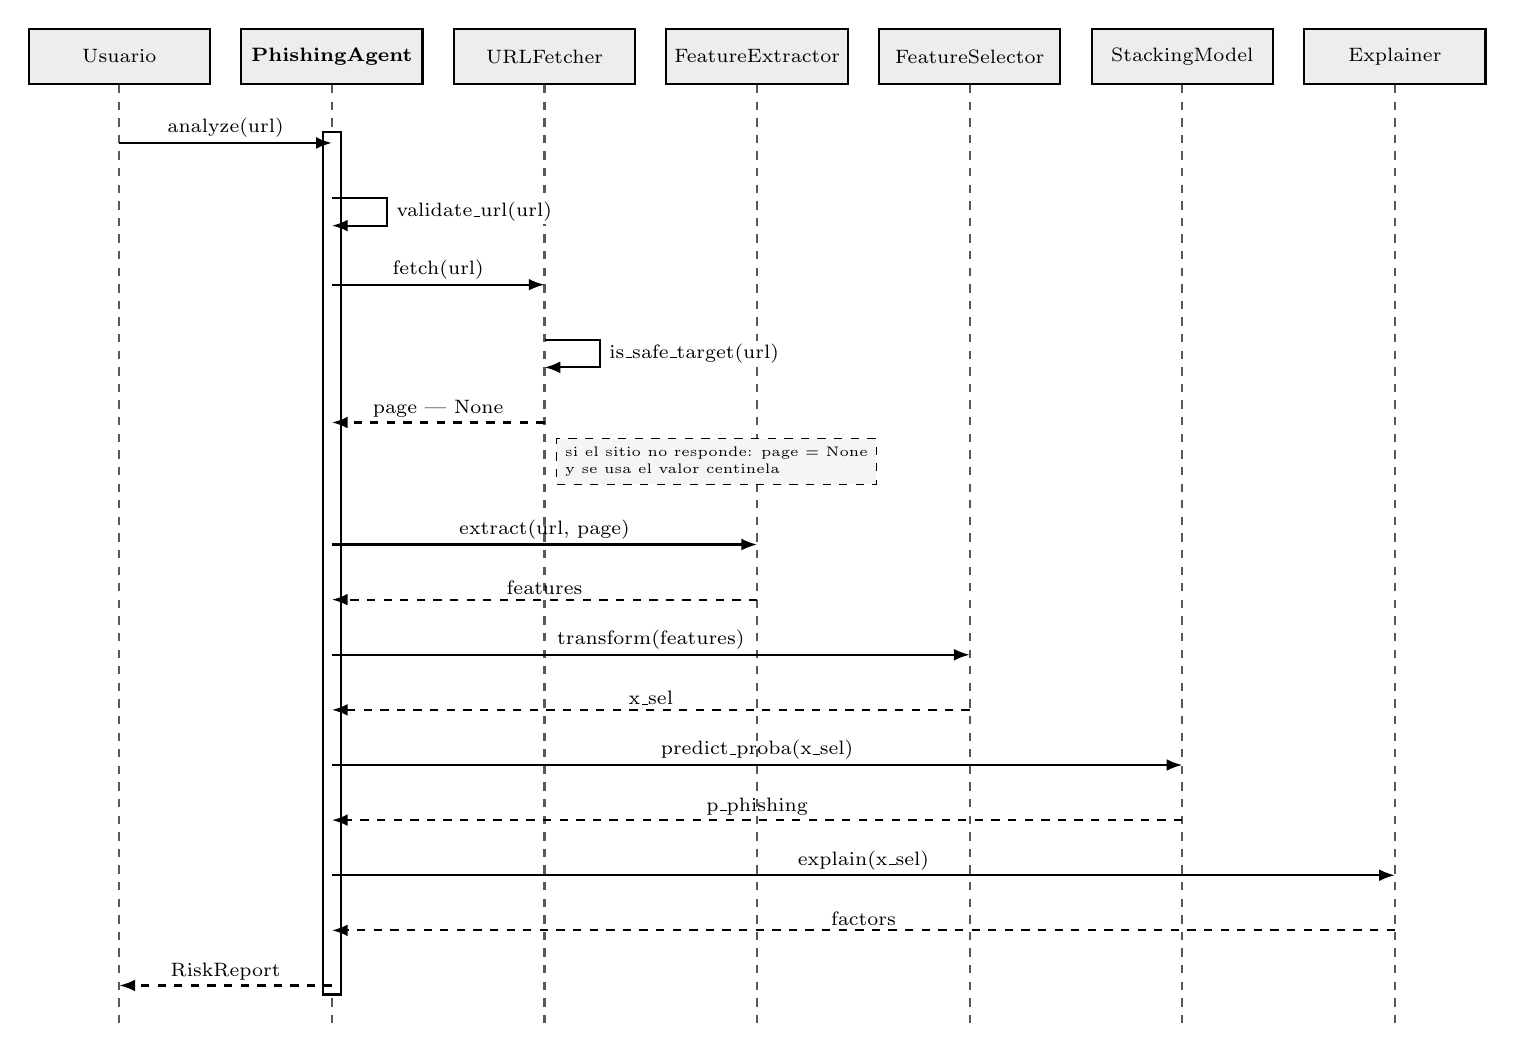
\begin{tikzpicture}[
    font=\scriptsize,
    vida/.style={rectangle, draw, thick, fill=gray!14, minimum width=2.3cm, minimum height=0.7cm, align=center, inner sep=3pt},
    linea/.style={dashed, gray!70!black, thick},
    msg/.style={-{Latex[length=2mm]}, thick},
    ret/.style={-{Latex[length=2mm]}, thick, dashed},
    et/.style={font=\scriptsize, inner sep=1.5pt},
    etw/.style={font=\scriptsize, inner sep=1pt, fill=white, anchor=west},
    act/.style={rectangle, draw, fill=white, thick, minimum width=0.18cm}
]
\def\dx{2.7}
\node[vida] (u)  at (0*\dx,0) {Usuario};
\node[vida] (a)  at (1*\dx,0) {\textbf{PhishingAgent}};
\node[vida] (f)  at (2*\dx,0) {URLFetcher};
\node[vida] (e)  at (3*\dx,0) {FeatureExtractor};
\node[vida] (s)  at (4*\dx,0) {FeatureSelector};
\node[vida] (m)  at (5*\dx,0) {StackingModel};
\node[vida] (x)  at (6*\dx,0) {Explainer};

\foreach \n in {u,a,f,e,s,m,x}{
  \draw[linea] (\n.south) -- (\n.south |- 0,-12.3);
}

\node[act, minimum height=10.95cm, anchor=north] at (a |- 0,-0.95) {};

\draw[msg] (u |- 0,-1.1) -- node[above, et]{analyze(url)} (a |- 0,-1.1);
\draw[msg] (a |- 0,-1.8) -- ++(0.7,0) -- ++(0,-0.35) -- ++(-0.7,0);
\node[etw] at ([xshift=0.78cm]a |- 0,-1.975) {validate\_url(url)};
\draw[msg] (a |- 0,-2.9) -- node[above, et]{fetch(url)} (f |- 0,-2.9);
\draw[msg] (f |- 0,-3.6) -- ++(0.7,0) -- ++(0,-0.35) -- ++(-0.7,0);
\node[etw] at ([xshift=0.78cm]f |- 0,-3.775) {is\_safe\_target(url)};
\draw[ret] (f |- 0,-4.65) -- node[above, et]{page | None} (a |- 0,-4.65);
\node[draw, dashed, fill=gray!8, align=left, font=\tiny, inner sep=3pt, anchor=north west]
   at ([xshift=0.15cm]f |- 0,-4.85) {si el sitio no responde: page = None\\ y se usa el valor centinela};
\draw[msg] (a |- 0,-6.2) -- node[above, et]{extract(url, page)} (e |- 0,-6.2);
\draw[ret] (e |- 0,-6.9) -- node[above, et]{features} (a |- 0,-6.9);
\draw[msg] (a |- 0,-7.6) -- node[above, et]{transform(features)} (s |- 0,-7.6);
\draw[ret] (s |- 0,-8.3) -- node[above, et]{x\_sel} (a |- 0,-8.3);
\draw[msg] (a |- 0,-9.0) -- node[above, et]{predict\_proba(x\_sel)} (m |- 0,-9.0);
\draw[ret] (m |- 0,-9.7) -- node[above, et]{p\_phishing} (a |- 0,-9.7);
\draw[msg] (a |- 0,-10.4) -- node[above, et]{explain(x\_sel)} (x |- 0,-10.4);
\draw[ret] (x |- 0,-11.1) -- node[above, et]{factors} (a |- 0,-11.1);
\draw[ret] (a |- 0,-11.8) -- node[above, et]{RiskReport} (u |- 0,-11.8);
\end{tikzpicture}}
\caption{Diagrama de secuencia del análisis de una URL. Las flechas continuas son llamadas y las discontinuas, respuestas.}
\label{fig:secuencia}
\end{figure*}


\subsubsection{Contrato de salida}

El agente siempre devuelve un RiskReport con los campos de la Tabla~\ref{tab:informe}, sin importar si el sitio estaba accesible o no. La etiqueta binaria sola le sirve poco a quien la recibe, así que el informe agrega la probabilidad, un nivel de riesgo legible, los factores que explican la decisión y una recomendación de mitigación asociada al nivel.\newline

El nivel de riesgo sale de aplicar umbrales a la probabilidad, se propone empezar con bajo por debajo de 0.30, medio entre 0.30 y 0.70, y alto por encima de 0.70, y ajustar esos valores con los datos de validación. Los umbrales hay que ajustarlos porque las probabilidades de XGBoost no están necesariamente calibradas, y un 0.93 no equivale a un 93\% de certeza real. La recomendación es un texto fijo por nivel, en riesgo alto, no ingresar credenciales ni datos personales, en medio, verificar el dominio por otra vía antes de interactuar, en bajo, que no se encontraron indicios fuertes, aclarando que eso no garantiza que el sitio sea seguro. Los campos missing\_features y factors hacen que el informe sea honesto con su propia incertidumbre, quien lo lee puede ver cuándo la predicción se hizo sin HTML.\newline

\begin{table}[ht]
\caption{Campos del informe de riesgo (\texttt{RiskReport}).}
\label{tab:informe}
\centering
\footnotesize
\renewcommand{\arraystretch}{1.15}
\begin{tabular}{p{2.4cm} p{5.5cm}}
\hline
\textbf{Campo} & \textbf{Contenido}\\
\hline
\texttt{url} & URL recibida, con los valores de los parámetros de consulta enmascarados\\
\texttt{final\_url} & URL final tras seguir las redirecciones\\
\texttt{label} & \texttt{phishing} o \texttt{legitimo}\\
\texttt{probability} & Probabilidad de phishing (0 a 1) del meta-clasificador\\
\texttt{risk\_level} & \texttt{bajo}, \texttt{medio} o \texttt{alto}, según umbrales sobre la probabilidad\\
\texttt{recommendation} & Texto de mitigación asociado al nivel de riesgo\\
\texttt{factors} & Las $k$ características con mayor contribución SHAP: nombre, valor observado y contribución con signo\\
\texttt{missing\_features} & Características que no pudieron calcularse (HTML o WHOIS no disponibles)\\
\texttt{model\_version} & Hash SHA-256 del artefacto del modelo usado\\
\hline
\end{tabular}
\end{table}


\subsubsection{Consideraciones de seguridad al analizar sitios sospechosos}

Analizar un sitio de phishing implica acercarse a algo hecho para hacer daño, y el propio agente es un blanco posible. Por eso el diseño asume que todo lo que viene de la red es no confiable y limita lo que el agente puede hacer con ello. La Tabla~\ref{tab:seguridad} resume los siete riesgos considerados y la medida que se toma contra cada uno. \newline

La decisión más importante es no ejecutar nada del sitio, no se usa un navegador, solo se descarga el HTML y se lo trata como texto. Esto tiene un costo, y es que el agente no ve contenido generado por JavaScript. Se acepta porque ejecutar páginas hostiles es justo lo que se quiere evitar. La otra medida es la validación del destino. Como el sistema corre en una máquina virtual en la nube, un atacante podría intentar que el agente consulte direcciones internas, como la del servidor de metadatos que suelen exponer esas máquinas. Por eso se rechazan IP privadas, de loopback y link-local, y la comprobación se repite en cada redirección, no solo en la URL inicial. \newline

El último riesgo de la tabla es el único que el diseño no puede resolver, el cloaking. Algunos sitios de phishing muestran contenido distinto a los clientes automáticos, de modo que un HTML sin formulario de login no prueba que el sitio sea legítimo. El modelo se apoya también en señales de la URL y del dominio, y el informe reporta qué características faltaron, pero esta limitación se discutirá de nuevo en la Evaluación.\newline

\begin{table}[ht]
\caption{Riesgos al analizar sitios sospechosos y medidas de diseño.}
\label{tab:seguridad}
\centering
\footnotesize
\renewcommand{\arraystretch}{1.15}
\begin{tabular}{p{2.4cm} p{5.5cm}}
\hline
\textbf{Riesgo} & \textbf{Medida}\\
\hline
Ejecutar código del sitio & Solo se descarga el HTML por HTTP y se analiza como texto; no se renderiza la página ni se ejecuta JavaScript\\
Acceso a recursos internos (SSRF) & Solo esquemas \texttt{http} y \texttt{https}; se resuelve el dominio y se rechazan IP privadas, de loopback y link-local (incluida 169.254.169.254); la validación se repite en cada redirección\\
Respuestas lentas o enormes & Tiempos límite de conexión y lectura, tope de bytes por descarga, máximo de redirecciones y longitud máxima de URL\\
Interacción con formularios & El agente solo lee los formularios: no los rellena ni los envía, y no manda cookies ni credenciales\\
Artefactos manipulados & El modelo se carga con \texttt{joblib}, que puede ejecutar código al deserializar; solo se cargan artefactos propios y se verifica su hash SHA-256 antes\\
Datos sensibles en la URL & Los parámetros de consulta se enmascaran en el informe y en los registros; WHOIS y DNS se consultan solo con el dominio\\
Cloaking & Un sitio puede mostrar otro contenido a clientes automáticos; la ausencia de un formulario no se toma como evidencia de legitimidad y las características faltantes se reportan\\
\hline
\end{tabular}
\end{table}

\subsection{Implementación}

El diseño anterior se implementa en un único notebook de Google Colab escrito en Python. Cada clase de la Figura~\ref{fig:clases} vive en su propia celda y se define una sola vez, de modo que se usa igual al entrenar y al analizar una URL nueva. A continuación se describen el entorno y las librerías, la correspondencia entre el diseño y el notebook, el entrenamiento y el guardado del modelo, la extracción de características en tiempo de ejecución, la explicabilidad con SHAP y las limitaciones que impone trabajar en Colab. Los fragmentos de código están recortados, pues son los que determinan el comportamiento del agente, no el notebook completo. \newline

\subsubsection{Entorno}

El notebook corre en un runtime de Colab solo con CPU. Los modelos son ensambles de árboles sobre unas veinte mil URLs y unas decenas de variables, así que no se necesita GPU. La primera celda instala con pip las librerías que Colab no trae, fija las semillas (random\_state=42 en todos los modelos y particiones) e imprime las versiones usadas, que se guardan en un requirements.txt en Drive Tabla~\ref{tab:librerias}. Registrar las versiones tiene una razón práctica, Colab actualiza sus librerías preinstaladas con el tiempo, y un modelo guardado con una versión puede fallar al cargarse con otra. Los recursos del runtime (CPU, RAM y disco) y el tiempo de cada etapa se registran con psutil y \%\%time, y se reportan junto con los resultados, porque Colab no garantiza los mismos recursos en cada sesión. \newline

\begin{table}[ht]
\caption{Librerías usadas en el notebook.}
\label{tab:librerias}
\centering
\footnotesize
\renewcommand{\arraystretch}{1.15}
\begin{tabular}{p{2.3cm} p{4.4cm} p{1.4cm}}
\hline
\textbf{Librería} & \textbf{Uso} & \textbf{Versión}\\
\hline
Python & Lenguaje del notebook & \textit{3.13.16}\\
pandas, numpy & Manejo de datos & \textit{2.2.3}\\
scikit-learn & Random Forest, \texttt{StackingClassifier}, \texttt{GroupKFold}, métricas & \textit{1.6.1}\\
xgboost & XGBoost en la capa 1 y como meta-clasificador & \textit{3.4.1}\\
lightgbm & Importancia de variables & \textit{4.6.0}\\
shap & Explicaciones por característica & \textit{0.54.1}\\
requests & Descarga HTTP & \textit{2.32.4}\\
beautifulsoup4 & Análisis del HTML & \textit{4.13.5}\\
python-whois & Antigüedad del dominio & \textit{0.9.6}\\
tldextract & Dominio registrable para agrupar las particiones & \textit{5.4.0}\\
joblib & Persistencia del modelo & \textit{1.6.0}\\
\hline
\end{tabular}
\end{table}

\subsubsection{Mapeo entre el diseño y el notebook}

El notebook se organiza en secciones que siguen el orden del diseño Tabla~\ref{tab:mapeo}. Las secciones 1 a 6 se ejecutan una sola vez para entrenar y guardar los artefactos. Las secciones 7 y 8 se pueden ejecutar solas en una sesión nueva, después de cargar esos artefactos desde Drive, y es lo que hace utilizable al agente sin reentrenar. Como cada clase se define una vez, el código de extracción que construye el dataset es el mismo que se ejecuta sobre una URL nueva, que era el objetivo del diseño. \newline

\begin{table*}[ht]
\caption{Correspondencia entre los módulos del diseño y las secciones del notebook.}
\label{tab:mapeo}
\centering
\footnotesize
\renewcommand{\arraystretch}{1.15}
\begin{tabular}{p{4.2cm} p{4.2cm} p{7.4cm}}
\hline
\textbf{Sección del notebook} & \textbf{Módulo del diseño} & \textbf{Función principal}\\
\hline
0. Configuración & Soporte & Instalar librerías, fijar semillas, montar Drive\\
1. Dataset & Entrenamiento & \texttt{build\_dataset()}: recolectar, deduplicar y registrar la fecha de captura\\
2. Adquisición & \texttt{URLFetcher} & \texttt{fetch()}, \texttt{is\_safe\_target()}\\
3. Extracción & \texttt{FeatureExtractor} & \texttt{extract()}: rasgos de URL, dominio y HTML\\
4. Selección & \texttt{FeatureSelector} & \texttt{fit()}, \texttt{transform()}: importancia promedio\\
5. Modelo y validación & \texttt{StackingModel} & \texttt{fit()}, \texttt{predict\_proba()}; validación con \texttt{GroupKFold}\\
6. Persistencia & Entrenamiento y Predicción & \texttt{save\_artifacts()}, \texttt{load\_artifacts()}\\
7. Agente & \texttt{PhishingAgent}, \texttt{RiskReport} & \texttt{analyze()}: orquesta el análisis y arma el informe\\
8. Explicabilidad & \texttt{Explainer} & \texttt{explain()}: contribuciones SHAP\\
9. Pruebas de evasión & Evaluación & URLs modificadas manualmente\\
\hline
\end{tabular}
\end{table*}

\subsubsection{Entrenamiento y persistencia del modelo}

La selección de características se implementa con tres modelos entrenados solo para medir importancia, XGBoost, LightGBM y Random Forest. Hay un detalle que cambia el resultado, XGBoost y Random Forest entregan importancias que ya suman 1, pero LightGBM, por defecto, devuelve cuántas veces se usó cada variable para dividir, es decir, conteos. Si se promedian tal cual, LightGBM domina el promedio. Por eso cada vector de importancias se normaliza antes de promediarlo. \newline

El apilamiento usa StackingClassifier de scikit-learn con stack\_method="predict\_proba". Esta clase entrena el meta-clasificador con predicciones fuera de muestra de los modelos base, no con las que esos modelos hacen sobre sus propios datos de entrenamiento. Sin eso, el meta-clasificador aprendería a confiar demasiado en modelos que ya vieron esas filas. En clasificación binaria, scikit-learn le pasa al meta-clasificador solo la probabilidad de la clase positiva de cada modelo base, de modo que recibe exactamente dos entradas, como lo plantea la Metodología. El meta-clasificador es un XGBoost deliberadamente pequeño de 50 árboles, profundidad 2; estos valores son iniciales y se ajustan con la búsqueda en grilla. \newline

La validación sigue la Metodología, GroupKFold de 10 particiones agrupando por dominio registrable (obtenido con tldextract), con la selección de variables y el balanceo calculados dentro de cada partición de entrenamiento. Al final se entrena el modelo con todos los datos y se guarda en Drive. \newline

Los artefactos son dos archivos, el modelo (model.joblib) y un manifest.json con las variables seleccionadas en su orden, el valor centinela, las versiones de scikit-learn y XGBoost, y el hash SHA-256 del modelo. Antes de cargarlo se recalcula el hash y, si no coincide con el del manifiesto, la carga se aborta. Esto atiende el riesgo de artefactos manipulados de la Tabla~\ref{tab:seguridad}, porque joblib puede ejecutar código al deserializar. Los primeros 12 caracteres del hash son el model\_version que aparece en el informe. \newline

\begin{figure*}[ht]
\begin{lstlisting}
def mean_importance(X, y, seed=42):
    modelos = [XGBClassifier(n_estimators=200, random_state=seed),
               LGBMClassifier(n_estimators=200, random_state=seed,
                              verbose=-1),
               RandomForestClassifier(n_estimators=200,
                                      random_state=seed, n_jobs=-1)]
    imps = []
    for m in modelos:
        m.fit(X, y)
        v = np.asarray(m.feature_importances_, dtype=float)
        imps.append(v / v.sum())      # LightGBM entrega conteos
    return pd.Series(np.mean(imps, axis=0),
                     index=X.columns).sort_values(ascending=False)

def build_stack(seed=42):
    return StackingClassifier(
        estimators=[("xgb", XGBClassifier(n_estimators=200,
                                          random_state=seed)),
                    ("rf", RandomForestClassifier(n_estimators=200,
                                                  random_state=seed,
                                                  n_jobs=-1))],
        final_estimator=XGBClassifier(n_estimators=50, max_depth=2,
                                      learning_rate=0.1,
                                      random_state=seed),
        stack_method="predict_proba", cv=5)

for tr, te in GroupKFold(n_splits=10).split(X, y, dominios):
    imp = mean_importance(X.iloc[tr], y[tr])
    sel = list(imp.index[:K])
    modelo = build_stack().fit(X.iloc[tr][sel], y[tr])
    evaluar(modelo, X.iloc[te][sel], y[te])

def save_artifacts(model, selected, path):
    path = Path(path); path.mkdir(parents=True, exist_ok=True)
    joblib.dump(model, path / "model.joblib")
    h = hashlib.sha256((path / "model.joblib").read_bytes()).hexdigest()
    vers = {p: md.version(p) for p in ("scikit-learn", "xgboost")}
    (path / "manifest.json").write_text(json.dumps(
        {"selected": selected, "sentinel": SENTINEL,
         "sha256": h, "versions": vers}))

def load_artifacts(path):
    path = Path(path)
    man = json.loads((path / "manifest.json").read_text())
    h = hashlib.sha256((path / "model.joblib").read_bytes()).hexdigest()
    if h != man["sha256"]:
        raise ValueError("el hash del modelo no coincide")
    return joblib.load(path / "model.joblib"), man
\end{lstlisting}
\caption{Selección por importancia promedio, apilamiento y persistencia con verificación de integridad.}
\label{lst:entrenamiento}
\end{figure*}

\subsubsection{Extracción de características en tiempo de ejecución}

URLFetcher descarga la página con la librería requests, y casi todo su código es para limitar lo que el sitio puede hacerle al agente. Los tiempos límite son de 3 segundos para conectar y 6 para leer, y hay además un tope total de 15 segundos, porque el límite de lectura de requests es por bloque recibido y un servidor lento que envía datos a cuentagotas podría mantener la descarga abierta indefinidamente. La respuesta se lee en streaming con tope de 2 MB, solo se acepta contenido HTML, y las redirecciones se siguen a mano (hasta 5) para poder validar cada destino antes de conectarse. Cualquier fallo (tiempo agotado, error de conexión, destino rechazado) se devuelve como un resultado con html = None y el motivo, nunca como una excepción que detenga el análisis. \newline

is\_safe\_target acepta solo los esquemas http y https, resuelve el nombre de dominio y rechaza el destino si alguna de las direcciones resueltas no es pública, con la propiedad is\_global de la librería ipaddress. Esa sola comprobación cubre las IP privadas, la de loopback y las link-local, incluida 169.254.169.254. Hay un riesgo residual que el prototipo no resuelve, la resolución de DNS se hace antes de la conexión, de modo que un servidor DNS hostil podría responder distinto la segunda vez (DNS rebinding). Cerrarlo exigiría conectarse directamente a la IP ya validada, lo que complica el manejo de HTTPS y queda fuera del alcance de este trabajo. \newline

La antigüedad del dominio se obtiene con python-whois y un tiempo límite de 5 segundos. La fecha de creación puede venir como una fecha, como una lista de fechas o sin zona horaria, así que se toma la más antigua y se normaliza a UTC. Si la consulta falla, por límite de consultas, por datos de registro ocultos o porque el dominio no tiene WHOIS, la función devuelve el valor centinela. WHOIS es la fuente más probable de valores faltantes. Del HTML descargado solo se conservan las características calculadas (por ejemplo, si hay un campo de contraseña y cuántos formularios tiene la página), y el HTML en sí se descarta. \newline

\begin{figure*}[ht]
\begin{lstlisting}
def is_safe_target(url):
    p = urlparse(url)
    if p.scheme not in ("http", "https") or not p.hostname:
        return False
    try:
        infos = socket.getaddrinfo(p.hostname, p.port or 443)
    except socket.gaierror:
        return False
    return all(ipaddress.ip_address(i[4][0]).is_global
               for i in infos)

def fetch(url, timeout=(3, 6), max_bytes=2_000_000,
          max_redirects=5, max_seconds=15):
    ua = {"User-Agent": "Mozilla/5.0 (PhishRiskAgent/0.1)"}
    limite = time.monotonic() + max_seconds
    try:
        for _ in range(max_redirects + 1):
            if not is_safe_target(url):
                return {"final_url": url, "html": None,
                        "error": "destino no permitido"}
            r = requests.get(url, headers=ua, timeout=timeout,
                             stream=True, allow_redirects=False)
            if r.is_redirect:
                url = urljoin(url, r.headers.get("Location", ""))
                r.close()
                continue
            if "html" not in r.headers.get("Content-Type", "").lower():
                r.close()
                return {"final_url": url, "html": None,
                        "error": "no es HTML"}
            datos = b""
            for trozo in r.iter_content(8192):
                datos += trozo
                if len(datos) > max_bytes or time.monotonic() > limite:
                    break
            r.close()
            html = datos[:max_bytes].decode(r.encoding or "utf-8",
                                            errors="replace")
            return {"final_url": url, "html": html, "error": None}
        return {"final_url": url, "html": None,
                "error": "demasiadas redirecciones"}
    except requests.RequestException as e:
        return {"final_url": url, "html": None, "error": type(e).__name__}

def domain_age_days(domain):
    try:
        c = whois.whois(domain, timeout=5).creation_date
        c = min(c) if isinstance(c, list) else c
        if c.tzinfo is None:
            c = c.replace(tzinfo=timezone.utc)
        return (datetime.now(timezone.utc) - c).days
    except Exception:
        return SENTINEL
\end{lstlisting}
\caption{Descarga con límites, validación del destino y antigüedad del dominio con valor centinela.}
\label{lst:extraccion}
\end{figure*}


\subsubsection{Explicabilidad con SHAP}

Sobre el modelo final completo, desde las variables seleccionadas hasta la probabilidad de phishing, se aplicará SHAP para generar dos tipos de explicación, una global, que muestra qué características pesan más en promedio sobre el dataset, y una local, que para una URL puntual muestra qué características empujaron la decisión hacia ``phishing'' o ``legítimo'' y en qué magnitud. Se explica el modelo completo y no solo el meta clasificador, porque este recibe únicamente las probabilidades de los dos modelos base y sus contribuciones no dirían nada sobre las características de la URL. La explicación local es la que responde directamente al objetivo de que la evaluación de riesgo venga acompañada de una justificación. \newline

Para datos tabulares y con un conjunto de fondo, la librería shap elige un explicador por permutaciones, que no depende del tipo de modelo y por eso sirve para el apilamiento completo. El fondo es una muestra de unas 50 filas de entrenamiento guardada junto al modelo. Las contribuciones salen en unidades de probabilidad y suman la diferencia entre la probabilidad de la URL analizada y la probabilidad media del fondo. Un valor positivo empuja hacia phishing y uno negativo, hacia legítimo. explain devuelve las top\_k variables de mayor contribución absoluta, con su valor observado y el signo de su contribución, que es el campo factors del informe. Para la explicación global se promedian las contribuciones absolutas sobre una muestra del conjunto de validación. El costo de cada explicación crece con el número de variables y el tamaño del fondo, y se medirá en la Evaluación. \newline

\begin{figure}[ht]
\begin{lstlisting}
class Explainer:
    def __init__(self, model, selected, background):
        self.sel = selected
        f = lambda d: model.predict_proba(
            pd.DataFrame(d, columns=selected))[:, 1]
        self.exp = shap.Explainer(f, background[selected])

    def explain(self, x, top_k=3):
        sv = self.exp(x[self.sel]).values[0]
        orden = np.argsort(-np.abs(sv))[:top_k]
        return [{"feature": self.sel[i],
                 "value": float(x[self.sel[i]].iloc[0]),
                 "shap": float(sv[i])} for i in orden]
\end{lstlisting}
\caption{Explicación SHAP sobre el pipeline completo.}
\label{lst:shap}
\end{figure}


\subsubsection{Limitaciones propias de Colab}

Sesiones efímeras. El runtime se recicla por inactividad o por tiempo máximo de uso, y con él se pierden las variables, el disco local y las librerías instaladas. Por eso el notebook se puede ejecutar de arriba abajo, instala sus dependencias al inicio y guarda en Drive todo lo costoso de recalcular, el dataset de características y los artefactos del modelo. \newline

Sin servicio persistente. Colab no permite dejar el agente encendido como una API con una dirección estable. El agente se usa de forma interactiva, llamando a analyze(url) desde el notebook. Convertirlo en un servicio (por ejemplo, una API pequeña en un servidor propio) o en una extensión de navegador queda como trabajo futuro. \newline

Recursos variables. CPU, RAM y tiempo disponibles no son los mismos en cada sesión, así que los tiempos medidos son indicativos y cada medición se reporta con las condiciones del runtime en que se hizo. \newline

Salida a Internet desde un centro de datos. Las peticiones salen desde direcciones de Google. Es probable que algunos sitios bloqueen esas direcciones o sirvan otro contenido a clientes automáticos, y que WHOIS limite las consultas, lo que aumenta la cantidad de características faltantes frente a un equipo doméstico. \newline

Versiones de librerías. Un modelo guardado puede no cargar tras una actualización de scikit-learn o XGBoost. El manifiesto guarda las versiones usadas y requirements.txt permite reproducir el entorno; si las versiones no coinciden al cargar, conviene reentrenar. \newline


\section{Discusión de Resultados}

Esta sección compara el agente con los trabajos revisados anteriormente, en cinco aspectos las condiciones experimentales, las técnicas y algoritmos, los resultados numéricos, el costo computacional junto con la explicabilidad, y la robustez frente a evasión. Una advertencia condiciona todo el análisis y es que ningún par de cifras es directamente comparable. Los trabajos \cite{kalabarige2022multilayer},\cite{kalabarige2023boosting},\cite{alsariera2020ai} se evalúan sobre datasets públicos cuyas características ya vienen calculadas, mientras que este proyecto construye su propio dataset a partir de URLs crudas. En cada comparación se indica qué parte de la diferencia puede atribuirse al modelo y cuál a los datos.

\subsection{Resultados obtenidos}

El dataset final tiene 19.989 URLs (10.000 de phishing y 9.989 legítimas) repartidas en 18.058 dominios. Casi todos los enlaces de phishing salieron de Phishing.Database (789.054 enlaces en la lista; OpenPhish aportó 300) y las URLs legítimas, de Tranco \cite{lepochat2019tranco}. Se apartó el 20\% de los dominios como prueba final (4.023 URLs) y las 15.966 restantes se usaron para ajustar hiperparámetros y elegir K. La búsqueda en grilla dejó XGBoost con 400 árboles, profundidad 6 y tasa de aprendizaje 0,05; Random Forest con 200 árboles y al menos 3 muestras por hoja; y un meta-clasificador de 30 árboles con profundidad 3. En la validación cruzada de 10 particiones la F1 del stacking casi no cambió al usar 17, 20, 23 o 26 variables (varió menos de 0,0015), de modo que se eligió K\,=\,0,6, es decir, 17 de las 29 variables. El experimento completo tomó 21,2 minutos en un runtime de Colab con 2 CPU y 13,6 GB de RAM. \newline

La Tabla~\ref{tab:resultados} resume el desempeño. El stacking obtiene la mejor exactitud y F1 en la prueba final, pero la diferencia con XGBoost solo es de 0,20 puntos porcentuales. Con 4.023 URLs el error estándar de una exactitud cercana a 0,91 es de 0,45 puntos (intervalo de confianza del 95\% de aproximadamente $\pm$0,9), y el de la diferencia entre dos modelos independientes, de unos 0,63 puntos. Es decir, la diferencia no se distingue del azar. No se aplicó una prueba pareada (por ejemplo, McNemar), que sería el siguiente paso para confirmarlo.

\begin{table}[t]
\caption{Desempeño de los modelos. Validación cruzada (10 particiones agrupadas por dominio, K\,=\,0,6, media) y prueba final (4.023 URLs apartadas).}
\label{tab:resultados}
\centering
\footnotesize
\setlength{\tabcolsep}{2.4pt}
\begin{tabular}{lcccccc}
\hline
\textbf{Modelo} & \textbf{Exact.} & \textbf{Prec.} & \textbf{Recall} & \textbf{F1} & \textbf{FPR} & \textbf{AUC}\\
\hline
\multicolumn{7}{l}{\textit{Validación cruzada (15,966 URLs)}}\\
Stacking      & 0,9099 & 0,9249 & 0,8923 & 0,9083 & 0,0725 & 0,9678\\
XGBoost       & 0,9090 & 0,9269 & 0,8880 & 0,9070 & 0,0700 & 0,9681\\
Random Forest & 0,9058 & 0,9152 & 0,8944 & 0,9047 & 0,0829 & 0,9637\\
\hline
\multicolumn{7}{l}{\textit{Prueba final (4,023 URLs)}}\\
Stacking      & 0,9123 & 0,9220 & 0,9014 & 0,9116 & 0,0768 & 0,9668\\
XGBoost       & 0,9103 & 0,9225 & 0,8965 & 0,9093 & 0,0758 & 0,9671\\
Random Forest & 0,9036 & 0,9117 & 0,8945 & 0,9030 & 0,0873 & 0,9634\\
\hline
\end{tabular}
\end{table}

\subsection{Condiciones experimentales y comparabilidad}

La Tabla~\ref{tab:literatura} reúne los datos y resultados de los trabajos revisados. Cuatro diferencias impiden leer las exactitudes de una columna contra otra. \newline

La primera es el origen de los datos. Los trabajos \cite{kalabarige2022multilayer},\cite{kalabarige2023boosting},\cite{alsariera2020ai} usan el dataset de UCI y las variantes de Mendeley, que se distribuyen con las características ya calculadas. Según \cite{alsariera2020ai}, 7 de las 30 características de UCI son de dominio, y entre ellas hay señales que dependen de servicios externos (en la documentación del dataset, el tráfico web y el PageRank). Algunos trabajos tratan esa dependencia de forma explícita, pues \cite{sahingoz2019machine} destaca que su sistema es independiente de servicios de terceros, y \cite{rao2019detection} evalúa su modelo con y sin ellos. En este proyecto las características salen de la URL, del HTML y de WHOIS, y esas señales externas no están disponibles. Además, en los datasets públicos las características se calcularon cuando los sitios estaban activos, mientras que aquí el 79,2\% de las URLs de phishing no devolvió HTML y el 64,0\% no devolvió datos de WHOIS. \newline

La segunda es el esquema de evaluación, pues \cite{alsariera2020ai} usa validación cruzada de 10 particiones aleatorias, y \cite{kalabarige2022multilayer,kalabarige2023boosting} no especifican la partición en el texto. Agrupar por dominio, como se hace aquí, tiene un efecto limitado en este dataset, porque hay 18.058 dominios para 19.989 URLs; por eso no explica por sí sola la diferencia de exactitud. Sí importa en otro punto, ya que en \cite{kalabarige2022multilayer} se describe el sobremuestreo aleatorio sobre el dataset completo y no aclara si ocurre antes o después de separar la prueba. Si fuera antes, copias de una misma fila quedarían en entrenamiento y en prueba, y la exactitud se inflaría. Con la información publicada no se puede saber. Este proyecto no necesitó balanceo, pues las clases quedaron casi iguales. \newline

La tercera es el conjunto de características, 29 aquí (17 tras la selección) frente a 30, 48 o 111 en los datasets públicos. \newline

La cuarta es el tamaño, 19.989 URLs, frente a unas 3.500 páginas en \cite{rao2019detection}, 11.055 en UCI o hasta 88.647 en las variantes de Mendeley de \cite{kalabarige2022multilayer}. \newline

El trabajo más cercano en condiciones es \cite{duy2024study}, ya que construye su dataset de sitios (23.960) con OpenPhish, PhishTank y Alexa, y sus clasificadores de sitios alcanzan entre 92,66\% y 94,58\% de exactitud (incluidos los que usan solo la URL), frente al 91,23\% de este proyecto. La revisión \cite{ahmad2025across} muestra el mismo patrón en general, donde las exactitudes de los modelos que compara van de 89\% a 99,6\%, y el valor depende en buena medida del dataset.

\begin{table*}[t]
\caption{Datos, evaluación y resultados reportados por los trabajos revisados. n.d.: no verificado (solo se consultó el resumen). Las exactitudes son las que cada trabajo reporta sobre sus propios datos.}
\label{tab:literatura}
\centering
\footnotesize
\renewcommand{\arraystretch}{1.15}
\setlength{\tabcolsep}{4pt}
\begin{tabular}{p{1.1cm} p{3.6cm} p{4.3cm} p{2.8cm} p{3.4cm}}
\hline
\textbf{Trabajo} & \textbf{Técnica principal} & \textbf{Datos y características} & \textbf{Evaluación} & \textbf{Exactitud reportada}\\
\hline
\cite{sahingoz2019machine} & Random Forest con características léxicas y de PLN & Más de 70.000 URLs; solo la URL, sin servicios de terceros & n.d. & 97,98\%\\
\cite{rao2019detection} & Random Forest y bosques oblicuos (PCA-RF) & Unas 3.500 páginas; URL, código fuente y servicios de terceros & n.d. & 99,31\% (RF); 99,55\% (PCA-RF)\\
\cite{chiew2019hybrid} & Selección HEFS y Random Forest & De 48 a 10 características (20,8\%) & n.d. & 94,6\%\\
\cite{zhu2019ofsnn} & Índice FVV y red neuronal & UCI, 23 de 30 características & n.d. & 94,5\% (valor tomado de \cite{kalabarige2023boosting})\\
\cite{aljofey2020effective} & CNN a nivel de carácter & Solo la URL & n.d. & 95,02\% (propio); 98,58, 95,46 y 95,22\% (públicos)\\
\cite{kalabarige2022multilayer} & Stacking de 3 capas (MLP, KNN, RF, LR, XGBoost) & UCI y Mendeley: 4 datasets (10.000 a 88.647 filas); sobremuestreo & No especifica & 96,79 a 98,90\%\\
\cite{kalabarige2023boosting} & Stacking de boosting con selección de variables & Los mismos 4 datasets, con 66 a 86\% de las variables & No especifica & 96,18 a 98,80\%\\
\cite{alsariera2020ai} & Extra-Trees con 4 meta-aprendices & UCI: 11.055 filas, 30 características & Validación cruzada de 10 particiones & 97,40 a 97,58\%\\
\cite{duy2024study} & 15 modelos (ML, ensamble, DL, multimodal) & 23.960 sitios de OpenPhish, PhishTank y Alexa; 220.423 dominios & n.d. & Sitios: 92,66 a 94,58\%; dominios: 89,00 a 99,74\%\\
\hline
\textbf{Aquí} & Stacking de XGBoost y Random Forest con meta XGBoost & 19.989 URLs crudas; 29 características (17 elegidas) & Validación cruzada de 10 particiones agrupada por dominio y 20\% apartado & 90,99\% (validación cruzada); 91,23\% (prueba final)\\
\hline
\end{tabular}
\end{table*}

\subsection{Técnicas, algoritmos y modelos matemáticos}

La Tabla~\ref{tab:tecnicas} compara las técnicas, los trabajos \cite{kalabarige2022multilayer}, \cite{kalabarige2023boosting},\cite{alsariera2020ai} y este proyecto comparten la idea de combinar árboles, pero cada uno usa una razón distinta para esperar una mejora. Random Forest promedia $B$ árboles entrenados sobre muestras distintas, $\hat{f}(x)=\frac{1}{B}\sum_{b=1}^{B} f_b(x)$, lo que reduce la varianza. Los métodos de boosting ajustan los árboles de forma secuencial y reducen el sesgo, donde AdaBoost combina clasificadores débiles con pesos $\alpha_m$, $H(x)=\mathrm{sign}\big(\sum_{m}\alpha_m h_m(x)\big)$, y XGBoost minimiza una función objetivo regularizada $\sum_i l(y_i,\hat{y}_i)+\sum_k \Omega(f_k)$ \cite{ahmad2025across}, por otro lado \cite{alsariera2020ai} fija un único algoritmo base (Extra-Trees) y varía la estrategia de combinación con remuestreo bootstrap en BET, reponderación de muestras en ABET, regresión logística aditiva en LBET y rotación por componentes principales en RoFBET. Mientras que en \cite{kalabarige2023boosting} se usa solo variantes de boosting, lo que reduce la diversidad entre modelos base. A su vez en \cite{kalabarige2022multilayer} se mezcla algoritmos de familias distintas (redes, vecinos, regresión y árboles), que es el caso con más diversidad. Este proyecto toma un punto intermedio con un modelo de boosting y uno de tipo bagging sobre las mismas variables, combinados por un meta-clasificador entrenado con predicciones fuera de muestra. Como ambos son ensambles de árboles que ven las mismas 17 variables, es plausible que sus errores se parezcan y que al meta-clasificador le quede poco por corregir. No se midió la correlación entre los errores, de modo que esto es una hipótesis y no un resultado. \newline

En la selección de variables el esquema es el de \cite{kalabarige2023boosting}, con un ajuste. El promedio de importancias de ese trabajo es $AVG_{F_i}=\frac{1}{n}\sum_j RF_i^j$. Aquí cada vector de importancias se normaliza antes de promediar,
\begin{equation}
\widetilde{AVG}_{F_i}=\frac{1}{3}\sum_{j=1}^{3}\frac{RF_i^{j}}{\sum_{k}RF_k^{j}},
\label{eq:avg}
\end{equation}
porque LightGBM devuelve por defecto el número de divisiones en que participa cada variable, y sin normalizar ese modelo dominaría el promedio. Frente a esto, en \cite{chiew2019hybrid} se deriva el subconjunto con un algoritmo de gradiente de la función de distribución acumulada y ensambles de perturbación de datos y de función, y en \cite{zhu2019ofsnn} se usa un índice de validez de las características (FVV). Ambos son más elaborados que fijar una fracción K por validación cruzada, y no hay evidencia aquí de que esa complejidad adicional compense, pues con tres modelos y un solo parámetro, la curva de F1 contra K resultó prácticamente plana. \newline

Donde este proyecto se diferencia de los trabajos revisados en detalle es en la explicabilidad. Puesto que en \cite{alsariera2020ai} se declara que sus modelos son interpretables, pero no muestra explicaciones por muestra, y en \cite{kalabarige2022multilayer,kalabarige2023boosting,duy2024study} devuelven solo una etiqueta o una probabilidad. Aquí cada informe incluye las variables que más pesaron, calculadas con valores de Shapley:
\begin{equation}
\phi_i=\sum_{S\subseteq F\setminus\{i\}}\frac{|S|!\,(|F|-|S|-1)!}{|F|!}\Big[f_{S\cup\{i\}}(x)-f_S(x)\Big],
\label{eq:shapley}
\end{equation}
con la propiedad de aditividad $\sum_i\phi_i=f(x)-E[f(X)]$: las contribuciones suman la diferencia entre la probabilidad de la URL y la probabilidad media del fondo. La contrapartida es que un modelo con variables diseñadas a mano depende de cómo se diseñaron, algo que en \cite{aljofey2020effective} se evita al aprender la representación directamente de los caracteres de la URL, a costa de perder la interpretación por variable. La sección sobre amenazas a la validez muestra que esa dependencia tuvo consecuencias aquí.

\begin{table*}[t]
\caption{Comparación de técnicas, selección de variables, fundamento matemático y explicabilidad. n.d.: no verificado (solo se consultó el resumen).}
\label{tab:tecnicas}
\centering
\footnotesize
\renewcommand{\arraystretch}{1.15}
\setlength{\tabcolsep}{4pt}
\begin{tabular}{p{1.3cm} p{2.7cm} p{3.0cm} p{2.5cm} p{3.6cm} p{2.3cm}}
\hline
\textbf{Trabajo} & \textbf{Algoritmos base} & \textbf{Combinación} & \textbf{Selección de variables} & \textbf{Fundamento principal} & \textbf{Explicabilidad}\\
\hline
\cite{kalabarige2022multilayer} & MLP, KNN, RF, LR, XGBoost & Stacking de 3 capas; meta XGBoost & No & Meta-aprendizaje sobre las salidas de cada capa & No\\
\cite{kalabarige2023boosting} & XGBoost, LightGBM, CatBoost, AdaBoost & Stacking de 3 capas solo de boosting & Importancia promedio; K de 66 a 86\% & $AVG_{F_i}=\frac{1}{n}\sum_j RF_i^j$ & No\\
\cite{alsariera2020ai} & Extra-Trees & AdaBoost, Bagging, Rotation Forest, LogitBoost & No & Bootstrap, reponderación, regresión logística aditiva, rotación PCA & Declarada, sin explicaciones por muestra\\
\cite{chiew2019hybrid}, \cite{zhu2019ofsnn} & Random Forest; red neuronal & --- & HEFS (gradiente de la CDF y ensambles de perturbación); índice FVV & Ranking de características con corte automático o por validez & n.d.\\
\cite{aljofey2020effective} & CNN a nivel de carácter & --- & No (aprende la representación) & Convolución sobre la secuencia de caracteres de la URL & n.d.\\
\cite{duy2024study} & 15 modelos de distintas familias & Atacados con WGAN; defensa por reentrenamiento & No & Pérdida de Wasserstein con recorte del crítico & No\\
\hline
\textbf{Aquí} & XGBoost y Random Forest (capa 1); XGBoost (meta) & Stacking de 2 niveles con predicciones fuera de muestra agrupadas por dominio & Importancia promedio normalizada (ec.~\ref{eq:avg}); K\,=\,0,6 & Boosting y bagging; valores de Shapley (ec.~\ref{eq:shapley}) & Sí, por URL (SHAP)\\
\hline
\end{tabular}
\end{table*}

\subsection{Comparación de resultados numéricos}

\textbf{Exactitud:} \par 

Con 91,23\% en la prueba final, el agente queda por debajo de los trabajos que usan datasets públicos (96,18 a 98,90\% en \cite{kalabarige2022multilayer,kalabarige2023boosting}, 97,40 a 97,58\% en \cite{alsariera2020ai}, 97,98\% en \cite{sahingoz2019machine}, 99,31\% en \cite{rao2019detection}). También queda entre 1,4 y 3,4 puntos por debajo de los clasificadores de sitios de \cite{duy2024study}, y esos incluyen tres modelos que usan solo la URL. Los resultados de \cite{chiew2019hybrid} (94,6\%), \cite{zhu2019ofsnn} (94,5\%) y \cite{aljofey2020effective} (95,02\% en su propio dataset, con solo la URL) también están por encima, aunque con menos margen. Dentro del rango de 89 a 99,6\% que muestra \cite{ahmad2025across}, el resultado cae en la parte baja. No hay una forma de repartir con exactitud la diferencia entre el modelo y los datos, pero la comparación con \cite{duy2024study}, donde las condiciones son parecidas, sugiere que la mayor parte viene de los datos, los datasets recolectados de fuentes activas producen cifras de 92 a 95\%, y los benchmarks con características curadas, de 96 a 99\%. \newline

\textbf{Tipo de error:} \par 
La tasa de falsos positivos es de 7,68\% (error estándar de 0,6 puntos), y el recall, de 90,14\%. En \cite{alsariera2020ai}, según sus tablas, los falsos positivos están entre 1,6 y 1,9\% y el recall entre 96,2 y 96,7\% (uno menos la tasa de falsos negativos). Dos trabajos que \cite{duy2024study} menciona reportan tasas de falsos positivos de 0,25\% y 0,59\%. Una de cada 13 URLs legítimas termina marcada como phishing, lo que haría poco usable al agente tal como está. El AUC de 0,967 indica que hay margen para mover el umbral de decisión y cambiar recall por menos falsos positivos, pero esa curva no se calculó. \newline

\textbf{Stacking frente a modelos individuales:} \par
La ganancia del stacking sobre XGBoost afinado es de 0,09 puntos en validación cruzada y 0,20 en la prueba final, dentro del error de medición. En \cite{kalabarige2023boosting} la ganancia sobre XGBoost con todas las variables va de 0,05 a 0,42 puntos según el dataset, un orden de magnitud parecido. En \cite{kalabarige2022multilayer} es mayor, de 0,20 a 1,08 puntos sobre el mejor modelo individual con las clases balanceadas y de 2,05 a 3,80 puntos sobre XGBoost sin balanceo. La brecha entre ambos trabajos sugiere que la ventaja del stacking depende de qué tan fuerte sea el modelo individual con el que se compara. Aquí XGBoost se ajustó con búsqueda en grilla, y con una línea base fuerte el beneficio casi desaparece. Para decidir si compensa el costo de entrenar tres modelos en lugar de uno, la evidencia disponible no alcanza para justificar el stacking. \newline

\textbf{Random Forest:} \par
Es el modelo individual más débil aquí (0,9036 de exactitud, 0,67 puntos por debajo de XGBoost), mientras que \cite{rao2019detection} lo reporta como el mejor y \cite{ahmad2025across} lo recomienda tras comparar modelos. Esa recomendación se apoya en cifras de datasets distintos, no en una comparación sobre los mismos datos, y en este dataset, con variables numéricas de URL y 20.000 filas, el boosting aprovecha mejor las interacciones entre variables. \newline

\textbf{Selección de variables:} \par 
Reducir de 23 a 17 variables no costó nada medible, lo que coincide con \cite{kalabarige2023boosting} (96,06 a 98,80\% con selección frente a 96,13 a 98,95\% sin ella en sus cuatro datasets) y con \cite{chiew2019hybrid}, que logra 94,6\% con solo el 20,8\% de las variables. La reducción aquí es menos agresiva (58,6\%). El promedio de importancias descartó variables binarias raras, como el uso de una dirección IP en lugar de un dominio (presente en el 1,8\% de las URLs de phishing y en ninguna legítima), que pueden ser decisivas en los pocos casos en que aparecen aunque su importancia media sea baja.\newline

\textbf{Qué señales pesan:} \par
Según SHAP, las cinco variables más importantes suman el 59,6\% de la importancia total: \texttt{uses\_https}, \texttt{num\_subdomains}, \texttt{digit\_ratio}, \texttt{path\_length} y \texttt{url\_length}. Las tres variables de contenido que quedaron entre las 17 (\texttt{num\_links}, \texttt{num\_scripts} y \texttt{has\_login\_form}) aportan el 5,9\%, y la de WHOIS (\texttt{domain\_age\_days}) ocupa el séptimo lugar. Es decir, el modelo funciona casi como un detector basado en la URL. Eso es coherente con \cite{sahingoz2019machine} y \cite{aljofey2020effective}, que alcanzan 95 a 98\% con solo la URL, pero significa que el componente de contenido, que era parte de la propuesta, casi no contribuye, algo esperable con el 80\% de las filas sin HTML.

\subsection{Costo computacional y explicabilidad}

El experimento completo (ajuste de hiperparámetros, validación cruzada con 4 valores de K y 3 modelos, y entrenamiento final) tomó 21,2 minutos en 2 CPU. Ninguno de \cite{kalabarige2022multilayer},\cite{kalabarige2023boosting},\cite{alsariera2020ai} reporta tiempos de entrenamiento, así que no hay referencia directa. Para una URL nueva, los tiempos medios medidos sobre 20 URLs de prueba fueron de 1,49 s para la descarga y WHOIS (mediana de 0,66 s, máximo de 6,79 s), 0,027 s para extraer las características, 0,061 s para la predicción y 1,25 s para la explicación. La predicción del modelo es, por tanto, la etapa más barata, y la explicación con SHAP cuesta unas 21 veces más que ella y casi iguala al tiempo de red, un análisis completo toma 2,83 s en promedio, frente a 1,58 s sin explicación. En \cite{duy2024study} se mide solo la predicción por lote de 1.000 sitios, con unos 1,1 ms por sitio para Fusion-CNN, 145 ms para Shark-Eyes y 238 ms para un modelo multimodal que usa URL, contenido y JavaScript; frente a esas cifras, los 61 ms de este modelo quedan por debajo de los dos multimodales y muy por encima de Fusion-CNN. El hardware y el método de medición difieren, por lo que sirven solo como orden de magnitud. El costo del agente es sobre todo de red y de explicación, no de modelo.

\subsection{Robustez frente a evasión}

La Tabla~\ref{tab:evasion} muestra qué fracción de 500 URLs de phishing, tomadas de las unas 1.820 que el modelo detecta sin modificar, sigue detectándose tras cada variante. Estas cifras no deben leerse como evidencia de robustez. Tres de las cinco variantes (subdominio extra, parámetros largos, dominio con caracteres cambiados) agregan señales que el modelo asocia con phishing, más subdominios, URLs más largas, más dígitos. Que se detecten casi todas era lo esperable. Las dos variantes que sí quitan señales son las más informativas, forzar HTTPS baja la detección al 95,4\%, y el acortador simulado, que deja la URL sin HTML ni WHOIS, al 90,4\%. La primera confirma que el modelo se apoya mucho en \texttt{uses\_https}, una característica que un atacante controla sin costo. \newline

\begin{table}[t]
\caption{Tasa de detección tras modificar 500 URLs de phishing ya detectadas. El acortador es una simulación (la URL queda sin HTML ni WHOIS).}
\label{tab:evasion}
\centering
\footnotesize
\begin{tabular}{lc}
\hline
\textbf{Variante} & \textbf{Tasa de detección}\\
\hline
Subdominio extra     & 1,000\\
Parámetros largos    & 0,996\\
Dominio con caracteres cambiados & 0,992\\
HTTPS forzado        & 0,954\\
Acortador simulado   & 0,904\\
\hline
\end{tabular}
\end{table}

Tampoco son comparables con \cite{duy2024study}, pues ahí un generador adversario produce dominios y solo se conservan los que logran pasar por un clasificador, de modo que el ataque está optimizado contra el detector; con esos ejemplos, el SVM detectó entre 10,02 y 13,67\% y XGBoost entre 19,24 y 38,32\% de los dominios, mientras que los modelos multimodales mantuvieron entre 95 y 99\%. Esa resistencia viene de que los modelos multimodales no dependen solo de la URL manipulada. El agente de este proyecto depende casi por completo de ella (94,1\% de la importancia está en variables de URL y dominio), de modo que su perfil es más parecido al de los modelos que usan solo la URL y que \cite{duy2024study} muestra como vulnerables (por ejemplo, entre 12 y 30\% de detección en Eman-CNN). La defensa que ese trabajo propone, reentrenar con ejemplos adversarios seleccionados, queda como trabajo futuro.

\subsection{Hallazgos que matizan los resultados}

La prueba del agente con una URL conocida mostró un problema que las métricas de la Tabla~\ref{tab:resultados} no revelan. \texttt{https://www.wikipedia.org/} fue clasificada como phishing con probabilidad 0,89 y riesgo alto. Los factores principales fueron \texttt{num\_subdomains} (+0.31, porque \texttt{www} cuenta como subdominio) y \texttt{path\_length} (+0.21, por la ruta \texttt{/}). Las URLs legítimas de este dataset salen de Tranco, que lista dominios sin \texttt{www}, y se construyeron como \texttt{https://dominio/}; las de phishing, en cambio, suelen incluir \texttt{www}. Los promedios por clase lo confirman en parte, pues \texttt{num\_subdomains} es 0,21 en legítimas y 0,57 en phishing, y \texttt{uses\_https} es 0,998 frente a 0,734. Esas dos variables son la primera y la segunda en importancia, y juntas suman el 29\% de la importancia total. Una parte de lo que el modelo aprendió es, por lo tanto, un artefacto de cómo se construyó la clase legítima, y como el mismo artefacto está en entrenamiento y en prueba, la exactitud de 91,23\% probablemente sobrestima el desempeño con URLs reales. Los trabajos con datasets curados \cite{kalabarige2022multilayer},\cite{kalabarige2023boosting},\cite{alsariera2020ai} no tienen este problema exacto, aunque tienen los suyos, y \cite{ahmad2025across} advierte que los modelos quedan atados al dataset con que se entrenaron. \newline

Hay otras limitaciones, como la igualación de valores faltantes entre clases que evita que el modelo aprenda que ``sin HTML'' significa phishing, pero no se midió su efecto con una comparación sin igualar. Las URLs se capturaron el mismo día, así que no se evalúa la generalización a sitios que aparecen después. Las URLs de phishing provienen casi todas de una sola fuente, y el desempeño por fuente no se separó. Las pruebas de evasión son simples y no adaptativas, y no se calcularon intervalos de confianza por bootstrap ni pruebas pareadas.

\subsection{Síntesis}

La comparación deja cuatro conclusiones. Primero, la exactitud de 91,2\% es menor que la de los benchmarks (96 a 99\%) y se parece a la de los trabajos que construyen su dataset con fuentes activas (92 a 95\%), por lo que la diferencia viene sobre todo de los datos y no solo del modelo. Segundo, el stacking no mejora de forma apreciable a XGBoost bien ajustado, en línea con las ganancias pequeñas que reporta \cite{kalabarige2023boosting}. Tercero, reducir las variables a poco más de la mitad no cuesta exactitud, como en \cite{kalabarige2023boosting} y \cite{chiew2019hybrid}, y el agente ofrece algo que no muestra ninguno de los trabajos revisados en detalle \cite{kalabarige2022multilayer},\cite{kalabarige2023boosting},\cite{alsariera2020ai},\cite{duy2024study}, una explicación por URL. Cuarto, el modelo depende de señales de URL que el atacante controla y de artefactos de la construcción del dataset, lo que limita lo que se puede afirmar sobre su robustez y sobre su uso con URLs reales. Corregir esos artefactos (quitar \texttt{www} del conteo de subdominios, muestrear el esquema de las legítimas según su frecuencia real) y volver a evaluar es el paso siguiente más útil.

\section{Conclusiones}

Este trabajo construyó un agente que recibe una URL cruda y estima su riesgo de phishing sin consultar listas de sitios ya reportados, y comparó sus resultados con los de la literatura revisada. Las conclusiones siguen los tres objetivos planteados. \newline

\textbf{Características asociadas al phishing:} \par 
Las señales que más separan las dos clases son léxicas y de dominio, el uso de HTTPS, el número de subdominios, la proporción de dígitos y la longitud de la URL, de la ruta y del nombre de host, junto con la edad de registro del dominio. Estas variables concentran el 94,1\% de la importancia SHAP de las 17 que conserva el modelo, mientras que las de contenido (enlaces, scripts y formularios de inicio de sesión) aportan el 5,9\%, algo esperable cuando el 79,2\% de las URLs de phishing ya no devolvía HTML. Reducir las variables de 29 a 17 no costó exactitud medible. Dos de las más importantes, el esquema HTTPS y el conteo de subdominios, reflejan en parte cómo se construyó la clase legítima y no una propiedad general del phishing. \newline

\textbf{Agente:} \par 
Se diseñó e implementó un agente con módulos separados (adquisición, extracción, selección, predicción, explicación e informe) que corre en Google Colab y entrega un informe con etiqueta, probabilidad, nivel de riesgo, factores explicativos y variables faltantes. Como el agente descarga páginas hostiles, el diseño limita lo que el sitio puede hacerle, no ejecuta JavaScript, rechaza destinos internos, acota el tiempo y el tamaño de la descarga y verifica la integridad del modelo antes de cargarlo. Sobre 4.023 URLs apartadas alcanzó 91,23\% de exactitud, F1 de 0,912 y AUC de 0,967. El stacking de XGBoost y Random Forest con meta-clasificador XGBoost superó a XGBoost solo por 0,20 puntos, una diferencia que no se distingue del error de medición y que coincide con las ganancias pequeñas que reporta \cite{kalabarige2023boosting}. Frente a un XGBoost bien afinado, apilar no se justificó por exactitud. \newline

\textbf{Utilidad para detectar, mitigar y pronosticar:} \par 
Para detectar, el agente sirve como apoyo y no como filtro autónomo, su tasa de falsos positivos es de 7,7\% (una de cada 13 URLs legítimas queda marcada) y clasificó como phishing a \texttt{https://www.wikipedia.org/}. Para mitigar, el aporte es el informe, pues cada resultado incluye una recomendación según el nivel de riesgo y las variables que lo motivaron, calculadas con valores de Shapley, algo que los trabajos revisados en detalle no ofrecen. Un análisis completo tarda 2,83 s en promedio, de los cuales 1,25 s corresponden a la explicación. Las recomendaciones son textos fijos y no se probaron con usuarios. Para pronosticar, el agente estima la probabilidad de que una URL desconocida sea phishing, pero no se midió su desempeño con sitios que aparecen después del entrenamiento, porque todas las URLs se capturaron el mismo día. Las pruebas de evasión fueron simples y no adaptativas, y la única que quita señales sospechosas (forzar HTTPS) bajó la detección a 95,4\%. \newline

\textbf{Alcance y trabajo futuro:} \par 
Las cifras no son comparables de forma directa con las de los trabajos que usan datasets públicos (96 a 99\%); se parecen más a las de quienes construyen su dataset con fuentes activas (92 a 95\%) \cite{duy2024study}. La exactitud probablemente está sobrestimada por los artefactos del dataset, y el agente solo analiza URLs públicas, las rutas protegidas y las direcciones internas se rechazan por seguridad. Como trabajo futuro, en orden de prioridad, se propone: 
\begin{itemize}
    \item Corregir los artefactos (no contar \texttt{www} como subdominio y muestrear el esquema de las legítimas según su frecuencia real) y reentrenar.
    \item Medir el efecto de igualar los valores faltantes y calcular la curva ROC para ajustar el umbral y reducir los falsos positivos.
    \item Evaluar con una partición temporal y con ataques adaptativos, incluida la defensa por reentrenamiento adversario de \cite{duy2024study}.
    \item Darle más peso al contenido de la página con una rama de análisis de HTML.
    \item Empaquetar el agente como servicio o extensión de navegador.
\end{itemize}

En conjunto, los resultados sugieren que un agente explicable de riesgo de phishing basado en la URL es viable con herramientas abiertas, y que su confiabilidad depende más de cómo se construyen los datos que del algoritmo elegido.

\bibliographystyle{IEEEtran}
\bibliography{bibliografia}
\end{document}
